\toftagthis{ceskekapely}
\song{Magdaléna}{Jelen}{40pt}{1}{
\verse{1}\A{}Zapal ten oheň ve mně,\D[add9]{} čeho se bojíš,\\
\A{}zápalkou škrtni jemně\D[add9]{}.\\
Zapal ten oheň ve mně, čeho se bojíš,\\
zimou se celá třeseš, proč venku stojíš?\\
Pojď \A{}dál, prosím tě, \D[add9]{}nenech se prosit se \A{}dál,\\
\D[add9]{}nenech se! 

\verse{2}Sedíme na pavlači, přichází ráno,\\
tobě se lesknou oči.\\
Sedíme na pavlači, přichází ráno\\
a mně se hlava točí.\\
Pojď dál, prosím tě, nenech se prosit se dál,\\
nenech se! 

\chorus{}\Fsm{}Hodiny se zastaví a v \E{}devět třicet v pondělí,\\
\A{}Magdaléno, \A{}tvoje vlasy\\
leží pod mou postelí a i když jsme to nechtěli,\\
oblíkáš se, pročpak asi.\\
Hodiny se zastaví a v devět třicet v pondělí\\
jsem\A{} sám.\D[add9]{}
\clearpage
\verse{3}Stojíme na rozcestí a zvony zvoní,\\
daleko od bolestí.\\
Stojíme na rozcestí a zvony zvoní,\\
možná nás čeká štěstí.\\
Pojď dál, prosím tě, nenech se prosit se dál,\\
nenech se!\\
\textbf{R:}

\chorus{}Hodiny se zastaví a v devět třicet v pondělí,\\
Magdaléno, tvoje vlasy,\\
leží pod mou postelí a i když jsme to nechtěli,\\
oblíkáš se, pročpak asi.\\
Hodiny se zastaví a v devět třicet v pondělí\\
máš těžký srdce a mokrý řasy,\\
když vycházíš ze dveří, tak sama tomu nevěříš,\\
nenech se!\\
}


\toftagthis{kabat}
\song{Malá dáma}{Kabát}{80pt}{0.955}{
\verse{1}\Am{}Utrhla trávu a začla \D[sus2]{}hrát,\\
ta malá dáma z předměs\F{}tí,\\
co umí \E[7]{}lidem z dlaní \Am{}číst.\\
Tam kočky z rána mívaj' hlad,\\
po noci plný neřestí\\
je pohladí a dá jim jíst.

\verse{*}\Dm{}Po tmě se \D[sus2]{}toulá a ve dne \Am{}spí\\
a její oči vědí víc než \Dm{}mý,\\
došly mi \D[sus2]{}slova, já stál tam \F{}jen,\\
s touhle \E[7]{}jedinou bych \Am{}zemřel.

\chorus{}\Am{}S touhle bych \F{}zemřel v jedinej \C{}den\\
a jestli \E[7]{}vám to\E[7sus4]{} ne - sta - \Am{}čí,\\
kdyby tam \F{}stála stovka \C{}žen,\\
vyzvu ji \E[7]{}k tanci, a to \E[+]{}netan\Am{}čím.

\verse{2}Tam za tratí svý doupě má,\\
mince po kašnách posbírá\\
a pak je skládá na kolej.\\
Staví si chrám, plechovej most,\\
už po něm kráčí první host,\\
tak ať ho nohy nebolej.

\verse{*}Prošla si peklem a kouzla zná,\\
přejetý mince počítá\\
a kdo ji spatří je zatracen,\\
s touhle jedinou bych zemřel.\\
\textbf{R:}


\hskip -7pt \verse{\Large Br}Budu si \Am{}pamatovat na tu \C{}chvíli,\\
když hrála, \F{}znělo to jak Paga\E[7]{}nini.\\
A já už \Am{}věděl, že jsem ztrace\C{}nej,\\
zeptal se \F{}za kolik, s pocitem \E[7]{}viny.\\
\textbf{R: ($2\times$)}
}


\toftagthis{nohavica}
\song{Malé české blues}{Jaromír Nohavica}{40pt}{1}{
\verse{1}{}Koupil jsem \Dm{}kozu, nemám kozu,\\
včera mi \G{}pošla na virozu,\\
kdybych koupil \Bb{}kozla, taky by mi \A{}chcip,\\
takový jsem \Dm{}cyp. \hskip 0.3em \A{}Do prdele práce!

\verse{2}{}Třešeň v rohu zahrady roky mi nesla,\\
letos úroda na polovinu klesla,\\
že prý špačci, já ti dám špačci,\\
snědí spoluobčané. Do prdele práce!

\verse{3}{}Dřu jak mezek ve zbrojovce,\\
ve volném čase za barákem chovám ovce,\\
Neuwirt chová rybky v akváriu,  má na kontě mega\\
a já nic. Do prdele práce!

\verse{4}{}Moje stará, škoda slov,\\
takový malý Suvorov,\\
jak mi liskne tak to třiskne jak když o traverzu\\
buchne těžký kov. Do prdele práce!\\
\clearpage
\verse{5}{}Starší dcera robí v Londonderry,\\
mladší čeká děcko, ale neví s kerym,\\
synek sedí, bo byl hlupy,\\
nechal se chytit. Do prdele práce!

\verse{6}{}Topolánek, jasné jak facka,\\
jezdí v plavkách do Chorvatska,\\
já tak možu na horní splav do Lidečka,\\
tečka. Do prdele práce!

\verse{7}{}Na posraného i hovno padá,\\  
tady je těžká jaká smysluplná rada,\\
nejlepší bude odložit bendžo a zajít na jedno.\\
Do restaurace --  tak já jdu.\\
}


\toftagthis{ceskekapely}
\song{Malování}{Divokej Bill}{20pt}{0.82}{
\crdheight=2.2ex
\verse{1}\Dm{}Nesnaž se, \Dm{}znáš se,\Bb{} řekni mi, \C{}co je jiný,\\
\Dm{} jak v kleci máš se\Bb{} \hskip 1.2em \C{}pro nevinný,\\
\Dm{}noci dlouhý \Bb{}jsou plný \C{}touhy a \Dm{}lásky nás dvou. \Bb{}\\
\C{}Všechno hezký \Dm{}za sebou mám,\Bb{} můžu \C{}si za to \Dm{}sám,\\
\Bb{} v hlavě \C{}hlavolam,\\
\Dm{}jen táta a máma\Bb{} jsou s \C{}náma, \Dm{}napořád s náma.\Bb{}

\vskip -2ex
\chorus{}To \C{}je to tvoje \Dm{}malování \Bb{}vzdušnejch z\C{}ámků,\\
\Dm{}malování po \Bb{}zdech holejma \C{}rukama tě \Dm{}nezachrání,\\
už \Bb{}máš na ka\C{}hánku, \Dm{}nezachrání, už jsi \Bb{}na zá\C{}dech,\\
je to \Dm{}za náma, ty čteš \Bb{}poslední str\C{}ánku,\\
\Dm{} za náma,\Bb{} na \C{}zádech, \Dm{}za náma, už \Bb{}máš na ka\C{}hánku,\\
mezi\Dm{} náma,\Bb{} mi taky \Gm{}došel \Am{}dech\ldots{} 

\Dm{} \hskip 2.1em \Bb{} \hskip 1.2em \C{} \hskip 1em \Dm{} \hskip 2.1em \Bb{} \hskip 1.2em \Gm{} \hskip 2em \Am{}\\
\textbf{R:}

\verse{2}Znáš se, řekni mi, co je jiný, jak v kleci máš se,\\
pro nevinný noci dlouhý jsou plný touhy a lásky nás tří.
}


\toftagthis{buty}
\song{Mám jednu ruku dlouhou}{Buty}{65pt}{0.85}{
\crdheight=2.2ex
\hskip 3em \revrpt{} \E{}Na \Csm{}nananana \A{}ná \E{}ná \rpt{}

\verse{1}{}\E{}Najdem si \Csm{}místo, \Gsm{}kde se dobře \Fsm{}kouří,\\
kde horké slunce do nápojů nepíchá,\\
\H{}kde vítr \H[/A]{}snáší \E{}šmolky ptačích \A{}hovínek\\
\H{}okolo \A{}nás a \H{}říká\ldots{}

\verse{2}{}Můžeme zkoušet, co nám nejvíc zachutná,\\
tak klidně se dívat jestli někdo nejde,\\
někdo, kdo ví, že už tady sedíme,\\
a řekne: \uv{Nazdar, kluci.}\\
\chorus{}\revrpt{} \E{}Mám \Csm{}jednu ruku \A{}dlou\E{}hou. \rpt{}

\verse{3}{}\A{}Posaď se \Fsm{}k nám, \Csm{}necháme tě \Hm{}vymluvit\\
a vzpomenout si na ty naše úkoly.\\
\E{}Tu ruku nám \Hm{}dej a \A{}odpočívej \D{}v pokoji \E{} \hskip 1em \E{} \\
\A{}tam na tom \Fsm{}místě, \Csm{}kde se dobře \Hm{}není. \E{} \hskip 1em \Fermataup{4}

\chorus{}\revrpt{} \A{}Na, \Fsm{}nananana \D{}ná \A{}ná \rpt{} $^{4\times}$\\
\revrpt{} \Am{}Na nananana \rpt{} $^{3\times}$  \D{}ná \A{}ná\\
\revrpt{} \A{}Mám \Fsm{}jednu ruku \D{}dlou\A{}hou. \rpt{} $^{4\times}$\\
}


\toftagthis{nohavica}
\song{Mám jizvu na rtu}{Jaromír Nohavica}{35pt}{0.83}{
\crdheight=2.3ex
\hskip 1em \revrpt{} \textsf{\bfseries Cadd9\ \ Gsus2/H\ \   Fsus2\ \ Gsus4 } \rpt{}

\verse{1}{}\C[sus2]{}Jsem příliš starý na to, abych věřil v revoluci,\\
\G[sus4]{}a svoji velkou hlavu \G{}těžko skryju \G[sus4]{}pod kapuci\\
\Am[7]{}a nechutná mi, když se \F[sus2]{}vaří předvařená rýže,\\
\C[sus2]v náprsní kapse nosím\G[sus4]{} Ventinol \G{}na potíže.

\vskip -2ex
\chorus{}\Am[7]{}Jak to tak vidím, asi těžko projdu \Am[7/E]{}uchem jehly\\
\F[sus2]{}a lesem běhám tak, a\C[sus2]{}by mě vlci nedoběhli,\\
\Dm[7]{}a kdyby se někdo z vás na anděla \C[/E]{}ptal,\\
tak \C[sus2]{}mám jizvu na rtu,\G[sus4]{} když při mně stál.

\verse{2}{}Sako mám od popílku, na kravatě saze,\\
mé hrubé prsty neumí uzly na provaze\\
a když mi občas tečou slzy, hned je polykám\\
a tančím jen tak rychle, jak hraje muzika.

\vskip -2ex
\chorus{}Mé oči mnohé viděly a ruce mnohé měly\\
a srdce stydělo se, když salvy slávy zněly,\\
a kdyby se někdo z vás na anděla ptal,\\
tak mám jizvu na rtu, když při mně stál.

\verse{3}{}Mluvil jsem s prezidenty, potkal jsem vrahy,\\
nahý jsem na svět přišel a odejdu nahý,\\
v patnácti viděl jsem, jak kolem jely ruské tanky,\\
a v padesáti nechával si věštit od cikánky.

\vskip -2ex
\chorus{}A dříve, než mě přijme svatý Petr u komise,\\
básníkům české země chtěl bych uklonit se\\
a kdyby se někdo z vás na anděla ptal,\\
tak mám jizvu na rtu, když při mně stál.

\verse{4}{}V Paříži četl jsem si ruskou verzi L'Humanité\\
a z bible zatím pochopil jen věty nerozvité,\\
v New Yorku chyt' jsem koutek od plastových lžiček,\\
ale nejlepší káva je v Hypernově U Rybiček.

\vskip -2ex
\chorus{}Trumfové eso v mariáši hážu do talónu\\
a chtěl bych vidět Baník, jak poráží Barcelonu\\
a kdyby se někdo z vás na anděla ptal,\\
tak mám jizvu na rtu, když při mně stál.

\verse{5}{}Někteří lidi mají fakt divné chutě,\\
ale já, lásko má, stále stejně miluju tě,\\
když hážeš bílé křemenáče na cibulku,\\
když zvedáš prst jako dirigentskou hůlku.

\vskip -2ex
\chorus{}A i když mě to táhne tam a tebe občas jinam,\\
na špatné věci pro ty dobré zapomínám\\
a kdyby se někdo z vás na anděla ptal,\\
tak mám jizvu na rtu, když při mně stál,\\
\ldots{} když při mně stál\ldots{} on při mně stál.\\
\noexport{
\vfill
\begin{figure}[h!]
\leftskip 5pt
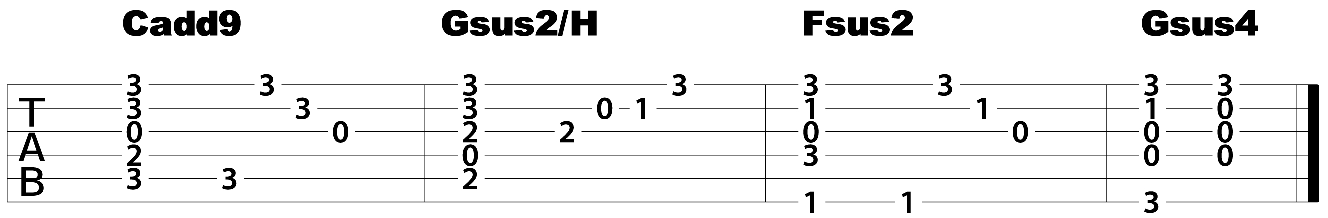
\includegraphics[width=345pt, height=60pt ]{res/jizvu.pdf}
\end{figure}
\leftskip 40pt
\rightskip 10pt
\hskip -50pt \begin{minipage}[t]{\textwidth} \chord{t}{x,p3,p5,p5,p3,p3}{Csus2} \end{minipage}
\hskip -15pt\begin{minipage}[t]{\textwidth}\chord{t}{p3,x,o,o,p1,p3}{Gsus4} \end{minipage}
\hskip -15pt\begin{minipage}[t]{\textwidth}\chord{t}{p3,x,o,o,o,p3}{G} \end{minipage}
\hskip -15pt\begin{minipage}[t]{\textwidth}\chord{t}{x,o,p2,o,p1,p3}{Ami7} \end{minipage}
\hskip -15pt\begin{minipage}[t]{\textwidth}\chord{t}{p1,x,p3,o,p1,p3}{Fsus2} \end{minipage}
\hskip -15pt\begin{minipage}[t]{\textwidth}\chord{t}{o,x,p2,o,p1,o}{C/E} \end{minipage}\\
}
}


\toftagthis{lucie}
\song{Medvídek}{Lucie}{80pt}{1}{
\verse{1}\A{}Dlouhá noc a mně se stýská moc,\\
pro tebe malý dárek mám.\\
Přes hory, \Hm{}přes ploty,\\
medvídek z \E[7]{}Bogoty už \A{}letí.  

\verse{2}Medvídek plyšový na cestě\\
křížový, Bůh ho ochrání\\
před smečkou \Hm{}římskejch psů\\
a jejich \E[7]{}úřadů\\
ti \D{}posílá lásku, co \E{}v bříšku má. 

\chorus{}\F{}Medvídek z Bogoty \A{}usnul a sní,\\
\F{}na kříži z Golgoty\A{} spí.\\
Za třicet \Hm{}stříbrných\\
z medvídka \E[7]{}padá sníh\\
no a ti \D{}římští psi\\
ho sjíždě\E{}jí na saních o Váno\A{}cích.
\clearpage
\leftskip 60pt
\verse{3}Nesvatá hodina medvídka proklíná,\\
že odhodil korunu bez trnů.\\
Medvídek ospalý pod křížem pokleká,\\
chce pít

\verse{4}Kalichem sladkosti medvídka\\
napustí do bříška, jak to má rád.\\
Koruna plyšová, vánoční cukroví,\\
nikdo se nedoví o svatozáři trnový.\\
\textbf{R:} 

\verse{*}\Am{}Medvídku, probuď se, \Am[/C]{}prober se, vstaň,\\
\Am[/F$\sharp$]{}psi se už \Am[/G]{}sbíhají, \Am[/E]{}připrav si dlaň,\\
slunce zas vychází, cítíš tu zář,\\
tlapky dáš v pěst, nebo nastavíš tvář. 

\Hm{}Římskejm psům a jejich \E{}úřadům\\
Maxipes \D{}Herodes vánoční \E{}slib dal dnes.\\
\textbf{R:}\\

}


\toftagthis{nohavica}
\song{Metro pro krtky}{Jaromír Nohavica}{70pt}{1}{
\verse{1}\G{}Prvá, druhá, \C{}třetí, \D{}čtvrtá,\G{} \hskip 1em \G{} \hskip 1em \C{} \hskip 1em \D{}\\
\G{}na za\G{}hradě \C{}krtek \D{}vrtá,\G{} \hskip 1em \G{} \hskip 1em \C{} \hskip 1em \D{}\\
\Em{} drápy \Em{}má jak \C{}výv\C{}rtky, oho\G{}ho,\\
\Am{} vrtá \Am{}metro \C{}pro krt\D{}ky, ohoho.\G{} \hskip 1em \G{} \hskip 1em \C{} \hskip 1em \D{}

\chorus{}Rrr ...

\verse{2}Každý, kdo si zaplatí, ohoho,\\
smí se projet po trati, ohoho,\\
od okurek po macešky, jé,\\
dál už musí každý pěšky, jé.

\chorus{}Rrr ...\\
}


\toftagthis{cechomor}
\song{Mezi horami}{Čechomor}{70pt}{1}{
\capo{5}
\verse{1}\revrpt{} \Em{}Mezi horami, lipka zelená, \rpt{}\\
\revrpt{} \G{}zabili Janka, \D{}Janíčka, \Em{}Janka\\
\Em{}miesto \D{}jele\Em{}ňa. \rpt{}

\verse{2}\revrpt{} Keď ho zabili, zamordovali, \rpt{}\\
\revrpt{}  na jeho hrobě, na jeho hrobě\\ 
kříž postavili. \rpt{}

\verse{3}\revrpt{} Ej, křížu, křížu, ukřižovaný, \rpt{}\\
\revrpt{}  zde leží Janík, Janíček, Janík\\ 
zamordovaný. \rpt{}

\verse{4}\revrpt{} Tu šla Anička plakat Janíčka, \rpt{}\\
\revrpt{}  hned na hrob padla a viac nevstala\\ 
dobrá Anička. \rpt{}\\
}

\toftagthis{nohavica}
\song{Mikymauz}{Jaromír Nohavica}{40pt}{0.9}{
\crdheight=2.3ex
\verse{1}\Am{}Ráno mě probouzí \G{}tma, sahám si na zápěs\F{}tí,\\
zda-li to \E{}ještě tluče, \Dm{}zda-li mám \E{}ještě štěstí,\\
\Am{}nebo je po mně a \G{}já mám voskované bo\F{}ty,\\
ráno co \E{}ráno stejné \Dm{}probuzení \E{}do nico\Am{}ty.

\vskip -2ex
\verse{2}Není co, není jak, není proč, není kam,\\
není s kým, není o čem, každý je v době sám,\\
vyzáblý Don Quijote sedlá svou Rosinantu\\
a Bůh je slepý řidič sedící u volantu.

\vskip -2ex
\chorus{}\E{}Zapínám \F{}telefon -- \Dm{}záznamník \E{}cizích citů,\\
špatné zprávy \F{}chodí jako \Dm{}policie, \E{}za úsvitu,\\
\Dm{}jsem napůl bdělý a \G[7]{}napůl ještě v noční pauze,\\
\C{}měl bych se smát, ale \E[sus4]{}mám ús\E{}měv Mikymauze,\\
\Am{}rána bych \Am[/G]{}zrušil. \hskip 1em \F{} \hskip 1em \E{} \hskip 1em \Am{}

\verse{3}Dobrý muž v rádiu pouští Čikoreu,\\
opravdu veselo je, asi jako v mauzoleu,\\
ve frontě na mumii mám kruhy pod očima,\\
růžový rozbřesk fakt už mě nedojímá.

\vskip -2ex
\verse{4}Povídáš něco o tom, co bychom dělat měli,\\
pomalu vychládají naše důlky na posteli,\\
všechno se halí v šeru, čí to bylo vinou,\\
že dřevorubec máchl mezi nás širočinou.

\leftskip 20pt
\chorus{}Postele rozdělené na dva suverénní státy,\\
ozdoby na tapetách jsou jak pohraniční dráty,\\
ve spánku nepřijde to, spánek je sladká mdloba,\\
že byla ve mně láska, je jenom pustá zloba,\\
dráty bych zrušil.

\verse{5}Prokletá hodina, ta minuta, ta krátká chvíle,\\
kdy věci nejsou černé, ale nejsou ani bílé,\\
kdy není tma, ale ještě ani vidno není,\\
bdění je bolest bez slastného umrtvení.

\vskip -2ex
\verse{6}Zběsile mi to tepe a tupě píchá v třísle,\\
usnout a nevzbudit se, nemuset na nic myslet,\\
opřený o kolena poslouchám tvoje slzy,\\
na život je už pozdě a na smrt ještě brzy.

\vskip -2ex
\chorus{}Co bylo kdysi včera, je, jako nebylo by,\\
káva je vypita a není žádná do zásoby,\\
věci, co nechceš, ať se stanou, ty se stejně stanou,\\
a chleba s máslem padá na zem vždycky blbou stranou,\\
máslo bych zrušil.

\verse{7}Povídáš o naději a slova se ti pletou,\\
jak špionážní družice letící nad planetou,\\
svlíknout se z pyžama, to by šlo ještě lehce,\\
dvacet let mluvil jsem a teď už se mi mluvit nechce.

\vskip -2ex
\verse{8}Z plakátu na záchodě prasátko vypasené\\
kyne mi, zatímco se kolem voda dolů žene,\\
všechno je vyřčeno a odnášeno do septiku,\\
jenom mně tady zbývá prodýchat pár okamžiků.

\vskip -2ex
\chorus{}Sahám si na zápěstí a venku už je zítra,\\
hodiny odbíjejí signály Dobrého jitra,\\
jsem napůl bdělý a napůl ještě v noční pauze,\\
měl bych se smát, ale mám úsměv Mikymauze,\\
\textls[-35]{rána bych zrušil\ldots{} lásku bych zrušil\ldots{} máslo bych zrušil.}\\
}


\toftagthis{filmove}
\song{Milenci v texaskách}{Starci na chmelu}{20pt}{1}{
\verse{1}\D{}Chodili spolu z čisté \Hm{}lásky \G{}a sedmnáct jim bylo \Hm{}let \hskip 1em \A[7]{}\\
\D{}a do té lásky bez nad\Hm{}sázky \G{}se vešel celý širý \Hm{}svět.\\
\G{}Ten svět v nich \Em{}ale viděl \Fsm{}pásky \G{}a jak by mohl nevi\A[7]{}dět,\\
\D{}vždyť horovali pro te\Hm{}xasky \G{}a sedmnáct jim bylo \Hm{}let.

\verse{2}A v jedné zvláště slabé chvíli, za noci silných úkladů,\\
ti dva se spolu oženili bez požehnání úřadů.\\
Ať vám to je či není milé, měla ho ráda, měl ji rád,\\
odpusťte dívce provinilé, jestli vám o to bude stát.

\verse{3}\D{}Ať vám to je či není \E[sus4/7]{}milé, \hskip 3em \G[maj]{} měla ho ráda, měl ji \H[sus2]{}rád\\
a bylo by moc pošetilé pro život hledat jízdní řád.\\
\textls[-9]{\G{}Tak jeden \Em[add9]{}mladík s jednou \Fsm{}slečnou \G{}se spolu octli na tra\A[7]{}ti,}\\
\D{}kéž dojedou až na ko\E[sus4/7]{}nečnou, \hskip 1em \G[maj]{}kéž na trati se nez\H[sus2]{}tratí,\\
\G[maj]{} kéž na trati se neztra\H[sus2]{}tí,\\
\G[maj]{} kéž na trati se neztra\H[sus2]{}tí\ldots{}
}


\toftagthis{nohavica}
\song{Milionář}{Jaromír Nohavica}{35pt}{0.9}{
U nás \D{}v domě říka\A[7]{}jí mi Franta \D{}Šiška,\D{}\\
bo už \D{}od pohledu \G{}chytrý jsem jak \D{}liška.\D{}\\
A když \D{}kery něco \Em{}neví nebo \A[7]{}když je na co \D{}levy,\\
tak jde \D{}za mnu a ja \A[7]{}všecko najdu \D{}v knižkach.\D{}\\
\D{} Ha \Em{}há, \hskip 0.5em \A[7]{}hahahá \D{}há,\\
tak jde \D{}za mnu a ja \A[7]{}všecko najdu \D{}v knižkach.\D{}

Raz mi říkal jeden známy dole v baře,\\
že s tu hlavu moh' bych do Milionaře.\\
Čemu ne, říkám si, brachu,\\
však má Železný dost prachu\\
no a Čechovi se podíváš do tváře.

Dostal jsem se mezi partu uchazeču.\\
Nikdo nemá šajnu jak tam nervy teču!\\
Všecko viděl jsem to hněde\\
tak jsem zmáčknul á, bé, cé, dé\\
no a už mě, kurva, ke stolečku vleču.

Čech to začal takým malým interiew,\\
co prý robim jestli kuřim a co piju.\\
Tak jsem řeknul, co jsem řeknul,\\
on se evidentně leknul\\
a už začly blikat světla ve studiu.\\

\leftskip -15pt
\large
\begin{minipage}[t]{0.54\textwidth}
\textls[-25]{První otázka, prý co je ukulele.\\
\textls[-55]{Tož to se přiznam měl jsem bobky u prdele.}\\
Tak jsem radši hlavu sklonil,\\
abych to všecko nezkonil,\\
říkám: \uv{Chtěl bych se obratit na přitele.}\\

Lojza byl po hlasu silně nevyspalý,\\
asi zase celu šichtu prochlastali.\\
Bylo slyšet, jak tam dycha,\\
ale třicet vteřin ticha.\\
To je tak, když se vam kamarád navali.\\

Moju staru zatím doma braly mory,\\
lidi ohryzávali televizory.\\
Tady nešlo nad čim plesat,\\
tož padesat na padesat,\\
ať vím, esi su to ty bulharské hory.\\

A už jasně na tym komputuře sviti:\\
buďto je to za A) vzácne lučni kviti,\\
nebo za B) nástroj strunny,\\
tu jde kurňa o koruny\\
a ja stejně jak na začátku jsem v řiti.\\

Čech tam zatím mával tymi svymi čisly.\\
Tak si řikam: Franta napij se a mysli.\\
Jake tudy sakypaky,\\
obratiš se na divaky,\\
však tu zatím za ty prachy enem kysli.}\\
\end{minipage}
\hskip 5pt
\begin{minipage}[t]{0.46 \textwidth}
\rightskip -25pt
\textls[-35]{Sám jsem byl zvědavý co publikum zvoli,\\
bo aj v obecenstvu možu sedět voli.\\
Devadesát procent za B),\\
ale to mi přišlo slabé,\\
bo co není stopro to mě dycky smoli.\\

Ještě že jsem chlap, co z boja neutika.\\
Říkám: \uv{Pane Čechu, pujdem do rizika.}\\
Měl jsem v gaťach nadělano,\\
ale Čech zakřičel: \uv{Ano,\\
máte pravdu, je to nástroj hudebnika!}\\
(Ha há, hahahá há, měl sem pravdu,\\
byl to nástroj hudebníka.)\\

Lidi tleskali, bo úspěch to byl plný.\\
Radosti zrobili dvě mexické vlny.\\
A já co mam srdce skromné,\\
jako všeci z Dolni Lomné,\\
jsem byl spokojený, bo sem ukol splnil.\\

\uv{\textls[-50]{Pane Čechu nerad přetáhnul bych strunu.}\\
Končim hru a beru tisicikorunu.}\\
Čech se jenom chytnul stolu,\\
obočí mu spadlo dolu\\
no a už se modry ku podlaze sunul.\\

První třidu do Ostravy Intercity.\\
V jidelňáku celu cestu valim kyty\\
a ta stovka co mi zbude,\\
to je přispěvek na chude,\\
bo Ostrava je region razovity.}
\end{minipage}
~\\
}

\toftagthis{nohavica}
\song{Milionář 2}{Jaromír Nohavica}{30pt}{1}{
\verse{1}Pane \D{}Nohavica, \A[7]{}znamý zpěva\D{}ku,\D{}\\
v živo\D{}tě jsem polknul \G{}křivdu kdeja\D{}ku,\D{}\\
ale \D{}to co vy jste \Em{}zrobil, tak to \A[7]{}jste mě fakt roz\D{}zlobil,\\
bo vy \D{}nemate cti \A[7]{}ani za ma\D{}ku.\D{}

\verse{2}Svévolně jste užil mého osudu,\\
zrobil jste ze mě hlupeho pobudu,\\
využil jste moji krize, jak jsem jel do televize,\\
v cele Dolní Lomné mám teď ostudu.

\verse{3}Stare baby, ba aj děcka nedospěle\\
po mně pokřikuji \uv{Franta ukulele!}\\
Zřekla se mě vlastní mama, musim chodit kanalama,\\
citim se jak sporťák Carda v TeleTele.

\verse{4}No a vy se zatím flákáte po TESCU,\\
mate velké auto, děcka, robu hezku,\\
za barakem modry bazen a ja stary cip a blázen\\
enem prazdnu kapsu a gatě na přezku.

\verse{5}Sto padesát tisíc prodaných cédeček,\\
tolik peněz, že se z toho chce až bečet,\\
natřískané kulturaky, baby ječí, chlapi taky,\\
no a za mnu se jen nouze s bídu vleče.

\verse{6}Napišu ten případ do krajského tisku,\\
že mě Nohavica okrad o část zisku,\\
buď se se mnou vyrovnáte, patřičný obnos mi dáte,\\
nebo dostanete u branky do pysku.

\verse{7}S úctou podepsany Franta Xaver Šiška,\\
sto osmdesát tři centimetrů výška,\\
boty dvanáct, vaha sto pět, jezdim v TIRu po Evropě\\
no a boxerky jsem dostal od Ježíška.\\
}


\toftagthis{zlutypes}
\song{Modrá}{Žlutý pes}{50pt}{1}{
\verse{1}\G{}Modrá je \D{}planeta, kde \C{}můžeme \D{}žít,\\
modrá je voda, kterou musíme pít,\\
modrá je obloha, když vodejde mrak,\\
modrá je \F{}dobrá, \C{}už je to \G{}tak.

\verse{2} Modrá je Milka -- ta naše kráva,\\
modrá je prej v Americe tráva,\\
modrá je údajně i polární liška,\\
senzačně modrá je moje vojenská knížka.

\chorus{}Jako \C{}nálada, když zahrajou poslední \G{}kus,\\
modrá je \F{}naděje, \C{}láska \F{}i moje \G{}blues.\\
Je to \C{}barva, kterou mám prostě \G{}rád,\\
modrá je \F{}dobrá, \C{}už je to \G{}tak.

\verse{3}Modrá je Raketa - ta moje holka,\\
modrá je vzpomínka na Mikyho Volka,\\
velká rána je modrej přeliv,\\
modrý voko má i černej šerif.\\
\textbf{R: $(2\times)$}

}

\toftagthis{folk}
\song{Montgomery}{Savana / tradicionál}{80pt}{0.94}{
\verse{1} \D{}Déšť ti, holka, smáčel \G{}vlasy, \Em{}\\
z \A[7]{}tvých očí zbyl prázdný \D{}kruh,\A[7]{}\\
kde je zbytek tvojí krásy,\\
to ví dneska jenom Bůh.

\chorus{}Z celé jižní eskadrony,\\
nezbyl ani jeden muž,\\
v Montgomery bijou zvony,\\
déšť ti smývá ze rtů růž.

\verse{2} Tam na kopci v prachu cesty,\\
leží i tvůj generál,\\
v ruce šátek od nevěsty,\\
ale ruka leží dál.\\
\textbf{R:}

\verse{3} Tvář má zšedivělou strachem,\\
zbylo v ní pár těžkých chvil,\\
proužek krve stéká prachem,\\
déšť mu slepil vlas jak jíl.\\
\textbf{R:}

\verse{4} Déšť ti šeptá jeho jméno,\\
šeptá ho i listoví,\\
lásku měl rád víc než život,\\
to ti nikdy nepoví.\\
\textbf{R:}\\
}


\toftagthis{kryl}
\song{Morituri te salutant}{Karel Kryl}{24pt}{0.87}{
\crdheight=2.3ex
\verse{1}Cesta je \Am{}prach a \G{}štěrk a \Dm{}udusaná \Am{}hlína\\
\C{}a šedé \F{}šmouhy \G[7]{}kreslí do vla\C{}sů\\
\revrpt{} a z hvězdných \F{}drah má \G{}šperk, co \C{}kamením se \E{}spíná,\\
\Am{}a pírka \G{}touhy z \Em{}křídel pega\Am{}sů. \rpt{}

\vskip -2ex
\verse{2}Cesta je bič, je zlá, jak pouliční dáma,\\
má v ruce štítky, v pase staniol\\
\revrpt{} a z očí chtíč jí plá, když háže do neznáma\\
dvě křehké snítky rudých gladiol. \rpt{}

\vskip -2ex
\chorus{}Seržante, \G{}písek je bílý, jak paže Daniely,\\
\Am{}počkejte chvíli, mé oči uviděly\\
\G[7]{}tu strašně dávnou vteřinu zapomnění,\\
\Am{}seržante, mávnou \G[7]{}a budem zasvěceni!\\
\C{}Morituri te salutant\E{}, morituri te salutant\ldots{}

\vskip -2ex
\verse{3}Tou cestou dál jsem šel, kde na zemi se zmítá\\
a písek víří křídla holubí\\
\revrpt{} a marš mi hrál zvuk děl, co uklidnění skýtá,\\
a zvedá chmýří, které zahubí. \rpt{}

\vskip -2ex
\verse{4}Cesta je tér a prach a udusaná hlína,\\
mosazná včelka od vlkodlaka,\\
\revrpt{} rezavý kvér -- můj brach a sto let stará špína\\
a děsně velká bíla oblaka. \rpt{}\\
\textbf{R:}
}



\toftagthis{anglicke}
\song{My Way}{Frank Sinatra}{30pt}{1}{
\capo{3}
\verse{1}And \G{}now, the end is \Hm[7/F$\sharp$]{}here,\\
and so I \Dm[6/F]{}face the final \E[7]{}curtain.\\
My \Am{}friend, I'll say it \Am[7/G]{}clear,\\
I'll state my \D[7/F$\sharp$]{}case of which I'm \G{}certain.\\
I've \G{}lived a life that's \G[7]{}full,\\
I traveled \C{}each and every \Cm{}highway\\
and \G{}more, much more than \D[7]{}this, I did it \Am[/G]{}my \hskip 2em \G{}way.

\verse{2}Regrets -- I've had a few,\\
but then again, too few to mention.\\
I did what I had to do\\
and saw it through without exemption.\\
I planned each charted course,\\
each careful step along the byway\\
and more, much more than this, I did it my way.

\chorus{}Yes, there were \G{}times, I'm sure you \G[7]{}knew,\\
when I bit \C{}off more than I could chew,\\
but through it \Am{}all, when there was \D[7]{}doubt,\\
I ate it \Hm{}up and spit it \Em{}out,\\
I faced it \Am{}all and I stood \D[7]{}tall and did it \Am[/G]{}my \hskip 2em \G{}way.

\verse{3}I've loved, I've laughed and cried,\\
I've had my fill, my share of losing.\\
And now, as tears subside,\\
I find it all so amusing.\\
To think I did all that\\
and may I say, not in a shy way,\\
\uv{Oh, no, oh, no, not me, I did it my way}

\chorus{}For what is a man, what has he got?\\
If not himself, then he has naught,\\
To say the things he truly feels\\
and not the words of one who kneels.\\
The record shows I took the blows and did it my way!
}
